%%%%%%%%%%%%%%%%%%%%%%%%%%%%%%%%%%%%%%%%%
% Beamer Presentation
% LaTeX Template
% Version 1.0 (10/11/12)
%
% This template has been downloaded from:
% http://www.LaTeXTemplates.com
%
% License:
% CC BY-NC-SA 3.0 (http://creativecommons.org/licenses/by-nc-sa/3.0/)
%
%%%%%%%%%%%%%%%%%%%%%%%%%%%%%%%%%%%%%%%%%

%----------------------------------------------------------------------------------------
%	PACKAGES AND THEMES
%----------------------------------------------------------------------------------------

\documentclass{beamer}


\mode<presentation> {

% The Beamer class comes with a number of default slide themes
% which change the colors and layouts of slides. Below this is a list
% of all the themes, uncomment each in turn to see what they look like.

%\usetheme{default}
%\usetheme{AnnArbor}
%\usetheme{Antibes}
%\usetheme{Bergen}
%\usetheme{Berkeley}
%\usetheme{Berlin}
%\usetheme{Boadilla}
%\usetheme{CambridgeUS}
%\usetheme{Copenhagen}
%\usetheme{Darmstadt}
%\usetheme{Dresden}
%\usetheme{Frankfurt}
%\usetheme{Goettingen}
%\usetheme{Hannover}
%\usetheme{Ilmenau}
%\usetheme{JuanLesPins}
%\usetheme{Luebeck}
\usetheme{Madrid}
%\usetheme{Malmoe}
%\usetheme{Marburg}
%\usetheme{Montpellier}
%\usetheme{PaloAlto}
%\usetheme{Pittsburgh}
%\usetheme{Rochester}
%\usetheme{Singapore}
%\usetheme{Szeged}
%\usetheme{Warsaw}

% As well as themes, the Beamer class has a number of color themes
% for any slide theme. Uncomment each of these in turn to see how it
% changes the colors of your current slide theme.

%\usecolortheme{albatross}
%\usecolortheme{beaver}
%\usecolortheme{beetle}
%\usecolortheme{crane}
%\usecolortheme{dolphin}
%\usecolortheme{dove}
%\usecolortheme{fly}
%\usecolortheme{lily}
%\usecolortheme{orchid}
%\usecolortheme{rose}
%\usecolortheme{seagull}
%\usecolortheme{seahorse}
%\usecolortheme{whale}
%\usecolortheme{wolverine}

\setbeamertemplate{footline} % To remove the footer line in all slides uncomment this line%

\setbeamertemplate{footline}[page number] % To replace the footer line in all slides with a simple slide count uncomment this line

%\setbeamertemplate{navigation symbols}{} % To remove the navigation symbols from the bottom of all slides uncomment this line
}

\usepackage{graphicx} % Allows including images
\usepackage{booktabs} % Allows the use of \toprule, \midrule and \bottomrule in tables

%----------------------------------------------------------------------------------------
%	TITLE PAGE
%----------------------------------------------------------------------------------------

\title[]{Visibility Driven Focus+Context Visualization of
Multimodal Volume Data} % The short title appears at the bottom of every slide, the full title is only on the title page

\author{M.Tech Thesis \\Srinivas R. Vaidya (MT2013152) \\
Supervisor: Prof. T K Srikanth } % Your name

\institute[IIITB] % Your institution as it will appear on the bottom of every slide, may be shorthand to save space
{International Institute Of Information Technology, Bangalore \\ % Your institution for the title page
\medskip
\textit{} % Your email address
}
\date{June 11, 2015} % Date, can be changed to a custom date


\begin{document}

\begin{frame}
\titlepage % Print the title page as the first slide
\end{frame}

\begin{frame}
\frametitle{Overview} % Table of contents slide, comment this block out to remove it
\begin{itemize}
\item Introduction
\item Non-photorealistic Rendering
\item Focus+Context for Volume Visualization
\item Related Work
\item Objective
\item Direct Volume Rendering Using Raycasting
\item Visibility Histogram
\item Transfer Function Design
\item Focus+Context for Multimodal Volume
\item Local Visibility Histogram
\item Implementation
\item Two-pass Volume raycasting
\item Future Work
\item References
\end{itemize}
\end{frame}

%----------------------------------------------------------------------------------------
%	PRESENTATION SLIDES
%----------------------------------------------------------------------------------------

%------------------------------------------------
\section{First Section} % Sections can be created in order to organize your presentation into discrete blocks, all sections and subsections are automatically printed in the table of contents as an overview of the talk
%------------------------------------------------

\subsection{Subsection Example} % A subsection can be created just before a set of slides with a common theme to further break down your presentation into chunks

\begin{frame}
\frametitle{Introduction}
\begin{itemize}
\item The aim of this thesis is to study mechanisms to improve focus+context visualization of multimodal volumetric data. \\ $ $
\item In particular use of visibility histograms is investigated. The technique described in Carlos and Ma [1] and Lin Zhend et al. [2] is analyzed. \\ $ $
\item Technique is demonstrated on multimodal data - CT and PET - to produce fused focus+context volume visualization. \\ $ $
\item We use ray tracing approach, which is implemented on GPU shaders to enable interactive response.

\end{itemize}
\end{frame}

%------------------------------------------------

\begin{frame}
\frametitle{Non Photorealistic Rendering}
\begin{itemize}
\item Non-photorealistic rendering(NPR) can be used to illustrate subtle spatial relationships that might not be visible with more realistic rendering techniques. \\ $ $
\item The integration of volume rendering with NPR is an intuitive and natural progression given the communicative and expressive capabilities of NPR. \\ $ $
\item Volume NPR techniques can be used to create visualizations of volume data that are more effective at conveying the structure within the volume. \\ $ $
\end{itemize}
\end{frame}

%------------------------------------------------

\begin{frame}
\frametitle{Focus+Context for Volume Visualization}
\begin{itemize}
\item Visualization of CT, MRI or PET data allows physicians and radiologists to see internal structures and organs with much greater detail.
\item In some cases there is too much data to be displayed at once on a computer display.
\item A simple and widely used solution is to zoom into specific region, and get lost in the dataset, resulting in loss of context, because we are no longer able to visualize the entire dataset.
\item Another approach to increase visibility of the specific region by making the occluding materials completely transparent. 
\item This brings focus to the region of interest, but, we could lose the context since the surrounding material or regions may become too transparent to provide meaningful information.
\end{itemize}
\end{frame}


%------------------------------------------------

\begin{frame}
\frametitle{Related work}
\begin{itemize}
\item Many techniques for multimodal visualization render the multi-volume by mixing the component volumes at a certain step of the volume rendering pipeline, such as, accumulation or at pixel levels[1]. \\ $ $
\item In another approach, one set of data and optical transformations are applied to the region of interest, and a different set of transformations to the remaining data.\\ $ $
\item Few other techniques include interactive cuts [3], opacity peelings [4]. \\ $ $
\item The technique of importance-aware rendering [5] and importance aware compositing [6], can help visual hidden structure. \\ $ $
\item But both these technique require prior definitions of context regions.
\end{itemize}
\end{frame}


%------------------------------------------------


\begin{frame}
\frametitle{Objective}
The objective of this thesis is to study techniques for viewing of volumetric data with the ability to support interactive and intuitive mechanisms for adjusting opacities of volume elements, such that it enhances visibility of structures or regions of interest to achieve  \textquotedblleft $\;$focus+context \textquotedblright.
\end{frame}

%------------------------------------------------

\begin{frame}
\frametitle{Overview Of Our Approach}

\begin{itemize}
\item Visibility, attemps to measure the impact of individual samples on the image generated by a volumetric object.\\ $ $
\item Visibility can be used to quantify the quality of transfer function  and ease their design towards more meaningful and efficient visualization. \\ $ $
\item Compute visibility histogram - is a representation of distribution of the visibility metric in relation to the domain values of the volume. \\ $ $
\item Visibility driven tranfser functions. \\ $ $
\item Implemented using Two-pass volume raycasting on GPU shaders. \\ $ $
\item We assume the volumes are uniform regular grids, and registration of volumes in multimodal visualization is done.

\end{itemize}

\end{frame}

%------------------------------------------------


\begin{frame}
\frametitle{Direct Volume Rendering using Raycasting}
\begin{itemize}
\item Volume rendering is a set of techniques used to display a 2D projection of a 3D discretely sampled data set, typically a 3D scalar field
\item Direct volume rendering involves generating visualizations without creating intermediate geometric structures, but simply by a direct mapping from volume data points to composited image elements.
\item Classification is a term that refers to assignment of optical properties to data values. Classification is one the most important steps in the volume rendering pipeline, since it is these optical properties that will either emphasize an feature or de-emphasize it.
\item The assignment of optical properties to data values is accomplished using a transfer function.
\end{itemize}
\end{frame}

%------------------------------------------------


\begin{frame}
\frametitle{Transfer Function}
\begin{itemize}
\item The role of the transfer function is to emphasize features in the data by mapping values and other data measures to optical properties. 
\item The simplest and most widely used transfer functions are one dimensional, and they map the range of data values to color and opacity.
\end{itemize}
\begin{figure}
\centering
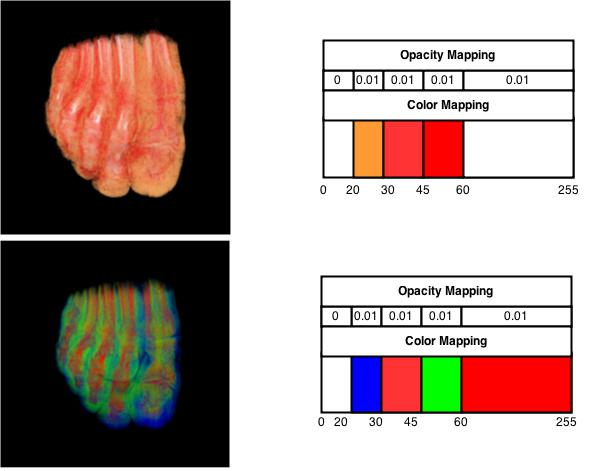
\includegraphics[width=150pt,heigth=280pt]{foot_different_TF.jpg}
\end{figure}
\end{frame}

%------------------------------------------------


\begin{frame}
\frametitle{Region of Interest}
A region of interest (often abbreviated ROI), is a selected subset of samples within a dataset identified for a particular purpose. A ROI can be any of the following: \\ $ $
\begin{itemize}
\item Volume of Interest. \\ $ $
\item A range of voxel intensities can also be a ROI. \\ $ $
\item A range of voxel intensities of one modality can be defined as an ROI in a multi-modal setup.
\end{itemize}
\end{frame}

%------------------------------------------------


\begin{frame}
\frametitle{Volume Ray Casting}
\begin{itemize}
\item Raycasting is a technique to visualize volume data. It is method in which for every pixel in the image, a ray is cast through the volume. \\ $ $
\item The ray intersects(or passes close to) a line of voxels. The color of the pixel is computed based on color and transparency of the voxels that are intersected by the ray.
\begin{figure}
\centering
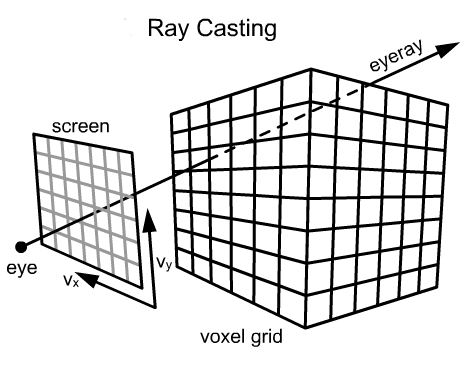
\includegraphics[width=150pt,heigth=280pt]{ray_cast1.jpg}
\end{figure}
\end{itemize}
\end{frame}

%------------------------------------------------


\begin{frame}
\frametitle{Volume Ray Casting -  Basic Algorithm}
\begin{itemize}
\item Generally, the volume is enclosed within a bounding primitive, a simple geometric object – usually a cuboid – that is used to intersect the ray of sight and the volume. \\ $ $
\item In general, the volume is not aligned with the ray of sight, and sampling points will usually be located in between voxels. Because of that, it is necessary to interpolate the values of the samples from its surrounding voxels. \\ $ $
\item After all sampling points have been fetched, they are composited along the ray of sight, resulting in the final color value for the pixel that is currently being processed.
\end{itemize}
\end{frame}


%------------------------------------------------

\begin{frame}
\frametitle{Sampling}
\begin{itemize}
\item Along the ray of sight within the volume at equidistant locations samples are selected. 
\item Generally, the volume is not aligned with the ray of sight, and sampling points will usually be located in between voxel's.
\item Because of that, it is necessary to interpolate the values of the samples from its surrounding voxels.
\item We have used trilinear interpolation.
\end{itemize}
\begin{figure}
\centering
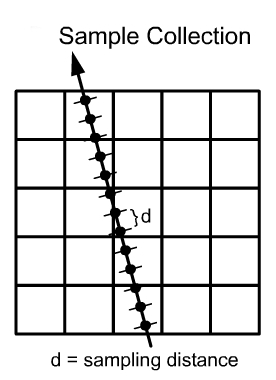
\includegraphics[width=50pt]{sampling1.jpg}
\end{figure}
\end{frame}

%------------------------------------------------

\begin{frame}
\frametitle{Compositing}
\textbf{Back-to-Front Compositing Equation}
\begin{itemize}
\item In this technique, samples are sorted in back-to-front order, and the accumulated color($\hat{C}_i $) and opacity($\hat{A}_i $) are computed iteratively.
\begin{equation}
\hat{C}_i \; = \; C_i \; + \; (1 \; - \; A_i ) \; \hat{C}_{i+1} 
\end{equation}
\begin{equation}
\hat{A}_i \; = \; A_i \; + \; (1 \; - \; A_i ) \; \hat{A}_{i+1} 
\end{equation}
\end{itemize}
\textbf{Front-to-Back Compositiong Equation}
\begin{itemize}
\item In this technique, samples are sorted in front-to-back order.
\item The composition is done towards the back and the current transparency is known at all times, the compositing can be stopped early when the opacity is above a threshold
\end{itemize}
\begin{equation}
\hat{C}_i \; = \; (1 \; - \; \hat{A}_{i-1} \; ) \; C_i \; + \; \hat{C}_{i-1}    
\end{equation}
\begin{equation}
\hat{A}_i \; = \; (1 \; - \; \hat{A}_{i-1} \; ) \; A_i \; + \; \hat{A}_{i-1}    
\end{equation}
\end{frame}

%------------------------------------------------


\begin{frame}
\frametitle{ Visibility}
\begin{itemize}
\item One of the limitations of contemporary visualization systems is the inability to quantify how visible a feature of interest is. \\ $ $
\item To be more effective, along with traditional transfer function design, visualization systems must also incorporate a measure of visibility. \\ $ $
\item Visibility metric, attemps to measure the impact of individual samples on the image generated by a volumetric object. It is measured as the contribution of a structure of interest to the final image. \\ $ $
\item Here, visibility can be used to quantify the quality of transfer function and ease their design towards more meaningful and efficient visualization. 
\end{itemize}
\end{frame}
%------------------------------------------------


\begin{frame}
\frametitle{Visibility Histogram}
\begin{itemize}
\item Visibility histograms provides intuitive cues to the user about the contribution of particular scalar values to the final image. \\ $ $
\item A visibility histogram is a representation of distribution of the visibility metric in relation to the domain values of the volume. \\ $ $
\item Samples are weighted by visibility and added into bins that partition the range of values in the scalar field. \\ $ $
\item for all sample values x in the volume.
\begin{equation}
VH[x] = VH[x] + ( 1 - AccumulatedOpacity ) Opacity(x) 
\end{equation}
\end{itemize}

\end{frame}
%------------------------------------------------


\begin{frame}
\frametitle{Visibility Histogram - Influence of the Transfer Function }
\begin{itemize}
\item Visibility histograms are transfer function dependent.
\end{itemize}
\begin{figure}
\centering
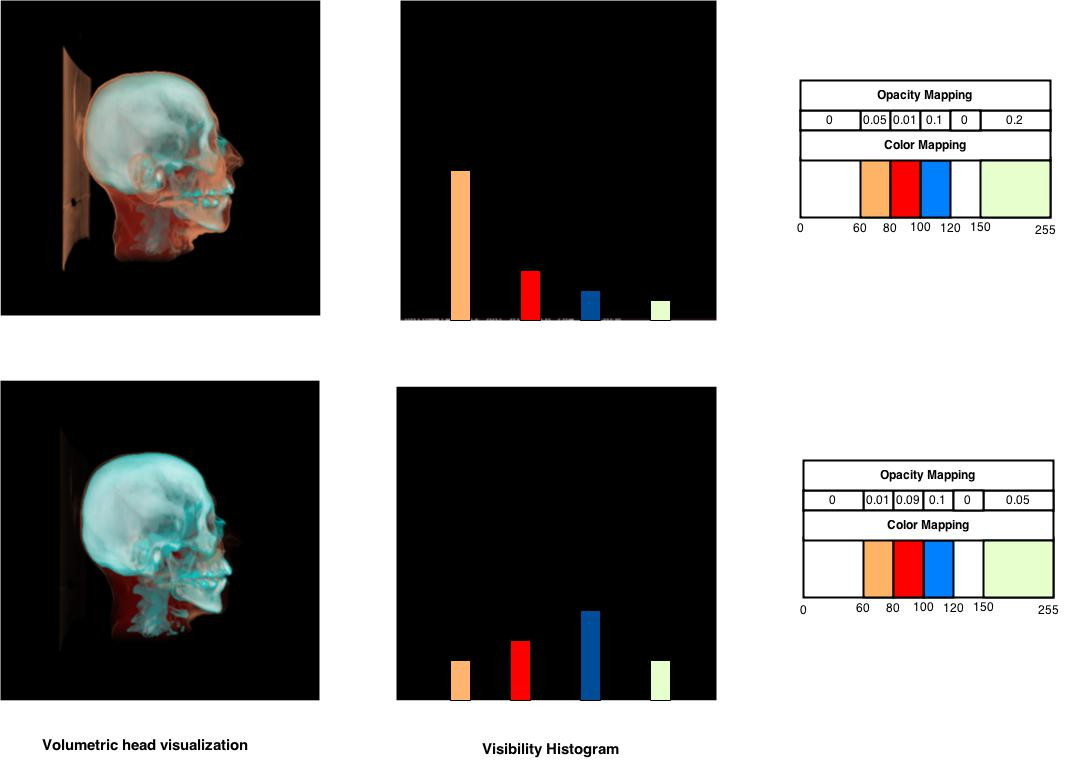
\includegraphics[width=200pt]{tf_influence.jpg}
\end{figure}
\end{frame}

%------------------------------------------------


\begin{frame}
\frametitle{Visibility Histogram - Influence of the Viewing Direction }
\begin{itemize}
\item A visibility histogram for a particular dataset is dependent on the direction from which the dataset is looked at, i.e. the direction of the viewing rays which traverse the data set.
\end{itemize}
\begin{figure}
\centering
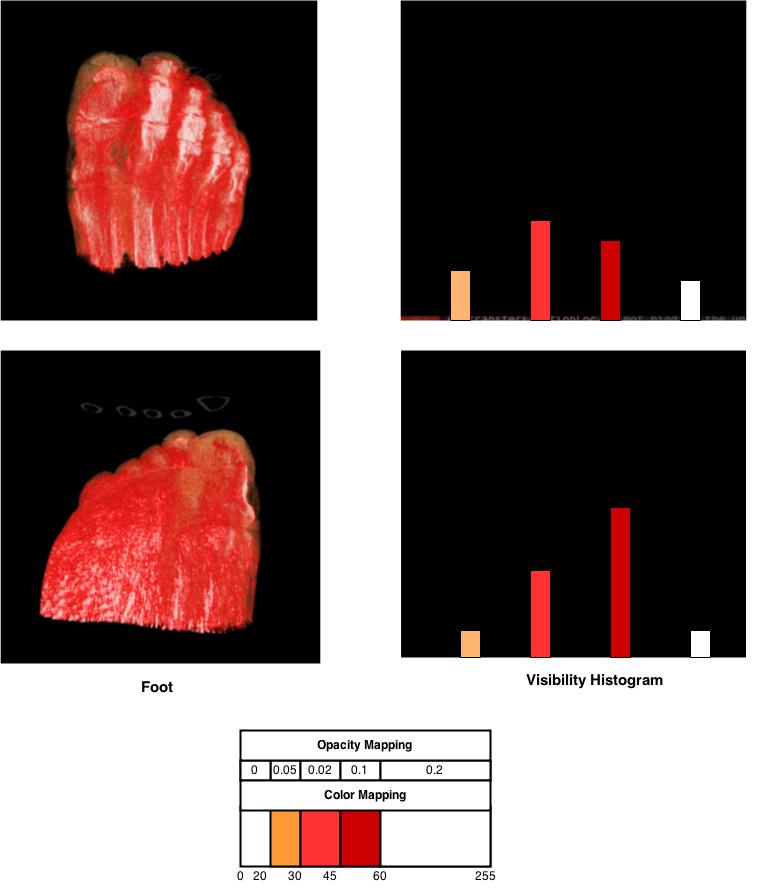
\includegraphics[width=150pt]{tf_view_influence.jpg}
\end{figure}
\end{frame}

%------------------------------------------------


\begin{frame}
\frametitle{Role Of Raycasting In Computing Visibility Histogram }
\begin{itemize}
\item Using the front-to-back compositing scheme
\end{itemize}
\begin{figure}
\centering
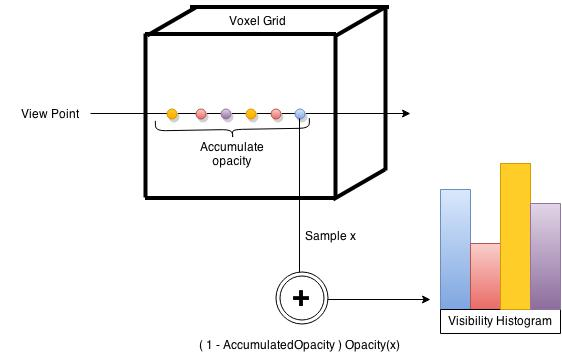
\includegraphics[width=200pt]{VHistogram.jpg}
\end{figure}
\end{frame}

%------------------------------------------------


\begin{frame}
\frametitle{Transfer Function Design}
Manually Generated Transfer Functions
\begin{figure}
\centering
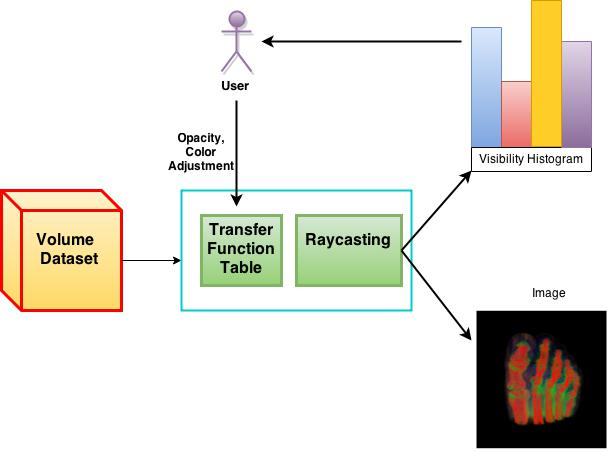
\includegraphics[width=250pt]{VH_pipeline.jpg}
\end{figure}
\end{frame}

%------------------------------------------------


\begin{frame}
\frametitle{Occulsion Signature}
The Visibility histogram helps find occulsion patterns.
\begin{figure}
\centering
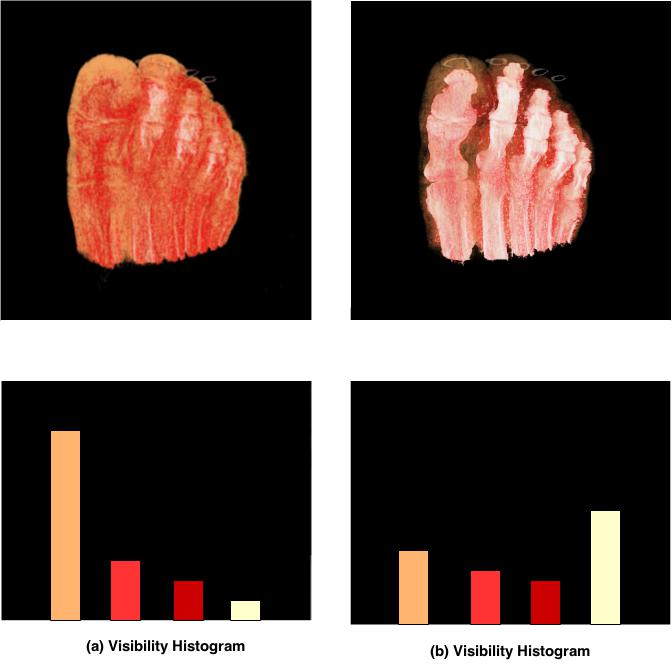
\includegraphics[width=200pt]{occlusion.jpg}
\end{figure}
\end{frame}

%------------------------------------------------


\begin{frame}
\frametitle{Focus+Context Using Visibility Histograms}
\begin{itemize}
\item A region of interest can be a range of voxel intensities. \\ $ $
\item Since range of voxel intensities define the ROI, visibility histogram can be used to find visibility of the ROI. \\ $ $
\item Using the visual cues from the Visibility Histogram, the user can modulate opacities to set the focus on ROI.  \\ $ $
\item Tradeoff between visibility and spatial clarity can be handled, by adjusting opacities of regions surrounding the ROI untill it meets user requirement.
\end{itemize}
\end{frame}


%------------------------------------------------


\begin{frame}
\frametitle{Context+Focus Visualization For Multimodal Volume}
\begin{itemize}
\item The advantage of using additional modalities is that they provide complementary or Supplementary information. \\ $ $
\item For example PET and CT dataset, PET data acts as the ROI we need to focus and CT data gives us the context. \\ $ $
\item One technical challenge that lies in multimodal dataset visualization is in ROI definition.  \\ $ $
\item One way would be set up a ROI around the structure of interest manually by identifying some key boundary points.
\end{itemize}
\end{frame}

%------------------------------------------------


\begin{frame}
\frametitle{Context+Focus Visualization For Multimodal Volume}
\begin{itemize}
 
\item If the structure is complex, user needs to define a larger number of boundary points around the ROI, which is time-consuming and error-prone. 
\item One solution to this problem is to define a sphere or bounding box covering the ROI
\item This solution is difficult to adopt, when the structure is complex, scattered or noisy.
\end{itemize}
\end{frame}

%------------------------------------------------

\begin{frame}
\frametitle{Approach for Multimodal Volume}
\begin{itemize}
\item Data set used are CT volume and fabricated PET volume, assuming registration is done. \\ $ $
\item Here, ROI is define as a range of voxel intensities of one modality in multi-modal setup. \\ $ $
\item Compute local histogram for rays hitting ROI and modulate opacities to achieve focus+context visualization. \\ $ $
\item Our approach in visualization of non-aligned volumes.
\end{itemize}
\end{frame}


%------------------------------------------------


\begin{frame}
\frametitle{Local Visibility Histogram}
\begin{itemize}
\item For those rays hitting the ROI, local histograms is computed for each ray
\item Rest of the rays cast into the volume are used to compute the global
histogram.
\item Using this, the user will now be able to manipulate the area of ROI, and
control the visibility of this area.
\end{itemize}
\begin{figure}
\centering
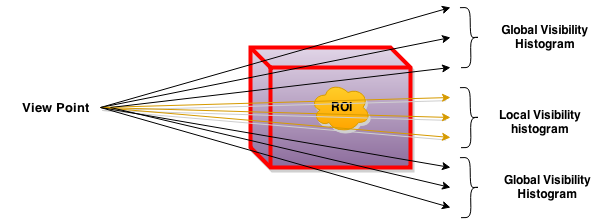
\includegraphics[width=250pt]{pet-ct-roi.png}
\end{figure}
\end{frame}


%------------------------------------------------


\begin{frame}
\frametitle{Local Visibility Histogram}
\begin{itemize}
\item Once visibility histogram is known, opacity of samples in the ROI are adjusted using the formula

\begin{equation} 
A^{'}(x) \; = \; A(x) \; ( \; 1 \; - \; VH(X) \; )^{e} 
\end{equation}

\item where, A($x$) and A$^{'}(x)$ are the old and new opacity mappings for intensity $x$.
\item VH($x$) is the visibility associated with that intensity in the visibility histogram.
\item $e$ is the exponent that defines the strength of such a mapping.
\item When VH($x$) is high(ie., it is more visible) it is likely to be made more transparent. 
\item When VH(x) is low, these samples do not occlude much and are retained to provide context. \\
\item This helps in keeping context clear which increasing the focus. 

\end{itemize}
\end{frame}


%------------------------------------------------


\begin{frame}
\frametitle{Effects of visibility-weighted adjustment e. }
\begin{figure}
\centering
e = 0    \hspace{50pt}      e = 1 \\
\vspace{3pt}
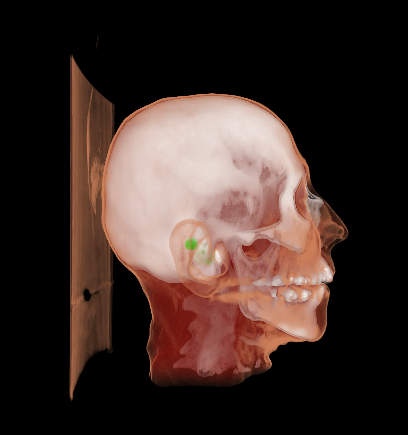
\includegraphics[width=80pt,height=80pt]{i=0.png}
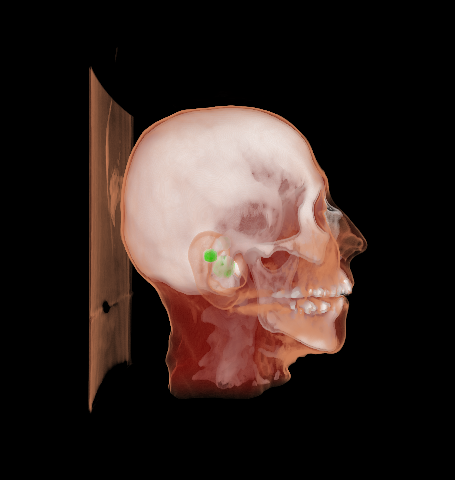
\includegraphics[width=80pt,height=80pt]{i=1.png}\\
e = 3    \hspace{50pt}      e = 10 \\
\vspace{3pt}
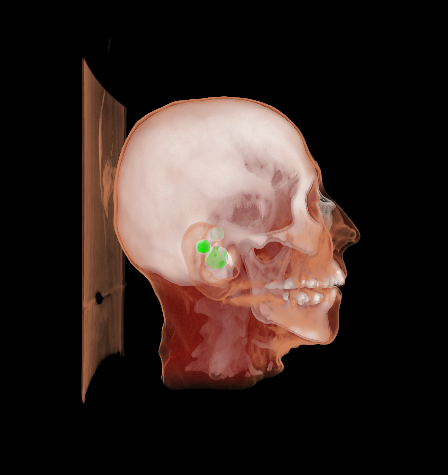
\includegraphics[width=80pt,height=80pt]{i=3.png}
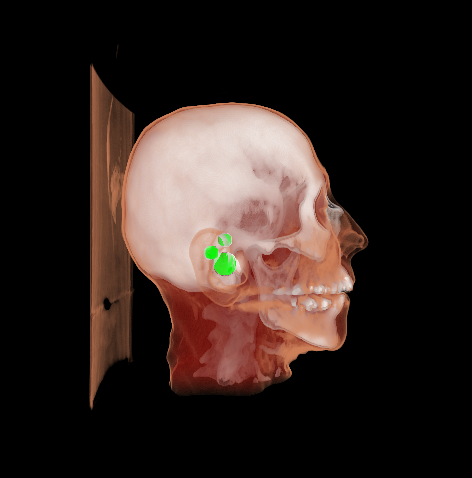
\includegraphics[width=80pt,height=80pt]{i=10.png}
\caption{Effects of visibility-weighted adjustment $e$. }
\end{figure}
\end{frame}
%------------------------------------------------


\begin{frame}
\frametitle{Volume ROI}
A region of interest can also be a volume, which is set of voxels within an 3D volume.
\begin{figure}
\centering
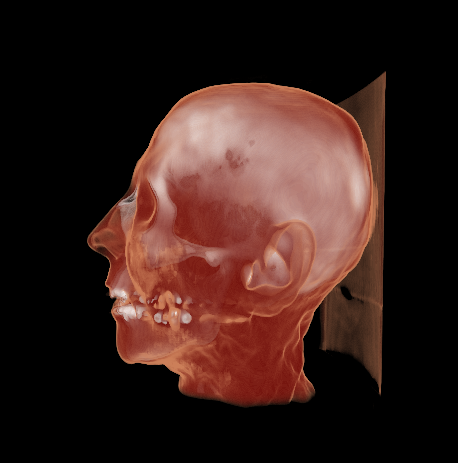
\includegraphics[height=120pt, width=120pt]{NON-VOI.png}
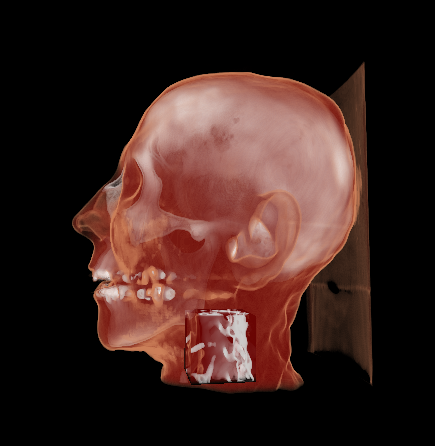
\includegraphics[height=120pt, width=120pt]{VOI.png}
\caption{\label{fig:ray_cast1.jpg} ROI bounded by a volume.}
\end{figure}
\end{frame}


%------------------------------------------------


\begin{frame}
\frametitle{Implementation}
\begin{itemize}
\item To perform raycasting on a volume for an arbitrary view direction, we need to compute the points at which each ray enters and exits the cube corresponding to the volume.
\item An efficient and convenient method for this is to render the front and back
faces of the cube into separate images.
\end{itemize}
\begin{figure}
\centering
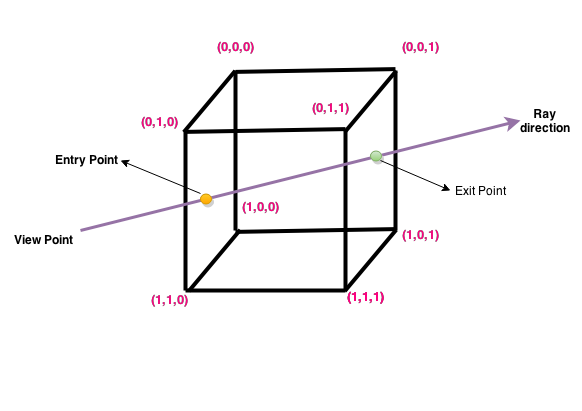
\includegraphics[width=160pt]{cube.png}
\caption{Assigning unique colors to all corners to the bounding box.}
\end{figure}
\end{frame}
%------------------------------------------------

\begin{frame}[fragile] % Need to use the fragile option when verbatim is used in the slide
\frametitle{Pseudocode of Two-pass Volume ray casting}
First pass: render the backface of the boundbox  \\
Second pass: render the frontface of the boundbox \\
Lookup volume exit position from backface 2D texture  \\
Entry position obtained at second pass    \\
Compute ray of sight direction  \\
While in volume  \\
\hspace{35pt} Lookup data value at ray position \\ 
\hspace{35pt} Apply transfer function to data value \\ 
\hspace{35pt} Accumulate color and opacity  \\
\hspace{35pt} Advance along ray\\
\end{frame}

%------------------------------------------------


\begin{frame}
\frametitle{Implementation }
\begin{itemize}
\item Implemented using OpenGL GLSL. \\ $ $
\item Computing Visibility Histogram. \\ $ $
\item Two-pass rendering using offscreen renderers. 
\end{itemize}
\end{frame}

%-------------------------------------------------------


\begin{frame}
\frametitle{Future work }
\begin{itemize}
\item We can incorporate lighting for better illustrative visualization. 
\item We can extend to two-dimensional transfer functions, for silhouette rendering in ROI and produce enhanced visualizations by incorporating NPR techniques. 
\item Volume raycasting and visibility driven transfer function techniques can also be used to visualize iso-surfaces of volumetric dataset. 
\item Enable visualization of non-uniform grids.
\item Study effects of integrating other NPR technique for multimodal visualization. 
\item Implementational aspects of the semi-automatic transfer function generation.
\end{itemize}
\end{frame}

%------------------------------------------------


\begin{frame}
\frametitle{Demonstration of Work done }
\begin{itemize}
\item Foot dataset \\ $ $
\item BostonTeapot \\ $ $
\item Head\_PET \\ $ $
\item Stent\_PET \\ $ $
\item Volume ROI
\end{itemize}

\end{frame}

%------------------------------------------------


\begin{frame}
\frametitle{References}
[1] Carlos D. Correa, Kwan-Liu Ma, "Visibility Histograms and Visibility-Driven Transfer Functions", IEEE Transactions on Visualization \& Computer Graphics, vol.17, no. 2, pp. 192--204, February 2011 \\ $ $
[2] L. Zheng, C. D. Correa, and K.-L. Ma. Visibility guided multimodal volume visualization. In In Proceedings of Bioinformatics and Biomedicine (BIBM), 2013 IEEE International Conference, pages 297–304, 12 2013. \\$ $
[3] W. Li, L. Ritter, M. Agrawala, B. Curless, and D. Salesin. Interactive cutaway illustrations of complex 3d models. ACM Trans. Graph., 26(3):31, 2007.\\$ $
[4]Z. Zhou, G. Wang, C. Huang, and H. Lin. Opacity modulation based peeling
for direct volume rendering. In Industrial Electronics and Applications (ICIEA), 2014 IEEE 9th Conference on, pages 1152–1157, June 2014. \\ $ $
[5] I. Viola, A. Kanitsar, and M. E. Gr”oller. Importance-driven feature enhancement in volume visualization. IEEE Transactions on Visualization and Computer Graphics, 11(4):408–418, 2005.

\end{frame}

%------------------------------------------------

\begin{frame}
\Huge{\centerline{Thank You!}}
\end{frame}

%----------------------------------------------------------------------------------------

\end{document} 
